\section{What is gpvdm?} 
Gpvdm stands for \emph{general purpose photovoltaic device model}.  As its name suggests it was originally developed to be a general purpose model for simulating photovoltaic devices, including organic and perovskite cells. However, since its initial development the model has expanded to simulate many other classes of optoelectronic devices including, Organic Light Emitting Diodes (OLEDs), Organic Field Effect Transistors (OFETs), large area printed devices, optical filters, photonic crystals and many more.  In general gpvdm can simulate any opto-electronic-device where electrons, photons (and also heat - phonons) interact.  Although the name no-loner really fits what gpvdm it has stuck as there are hundreds of papers which cite gpvdm, and it has been downloaded by thousands of people across the globe (see figure \ref{fig:downloadmap}) it therefore no longer makes sense to update the name.

Figure \ref{fig:alldevices} shows some of the classes of devices gvpdm can simulate. The model should be though of as a general, 1/2D electrical drift-diffusing solver, combined with a 3D thermal solver and advanced optical models.  The thermal model is 3D so is the exciton diffusion model.  The key feature which sets gpvdm apart from many other models is the efficient way it handles SRH carrier trap states. 

Gpvdm is written in small letters because its a UNIX command like \href{https://en.wikipedia.org/wiki/Grep}{grep}, it is permissible to write it with a capital letter at the start of a sentence, but it should \emph{never} be fully capitalized as GPVDM.

%\begin{wrapfigure}{r}{0.5\textwidth}
%  \begin{center}
%    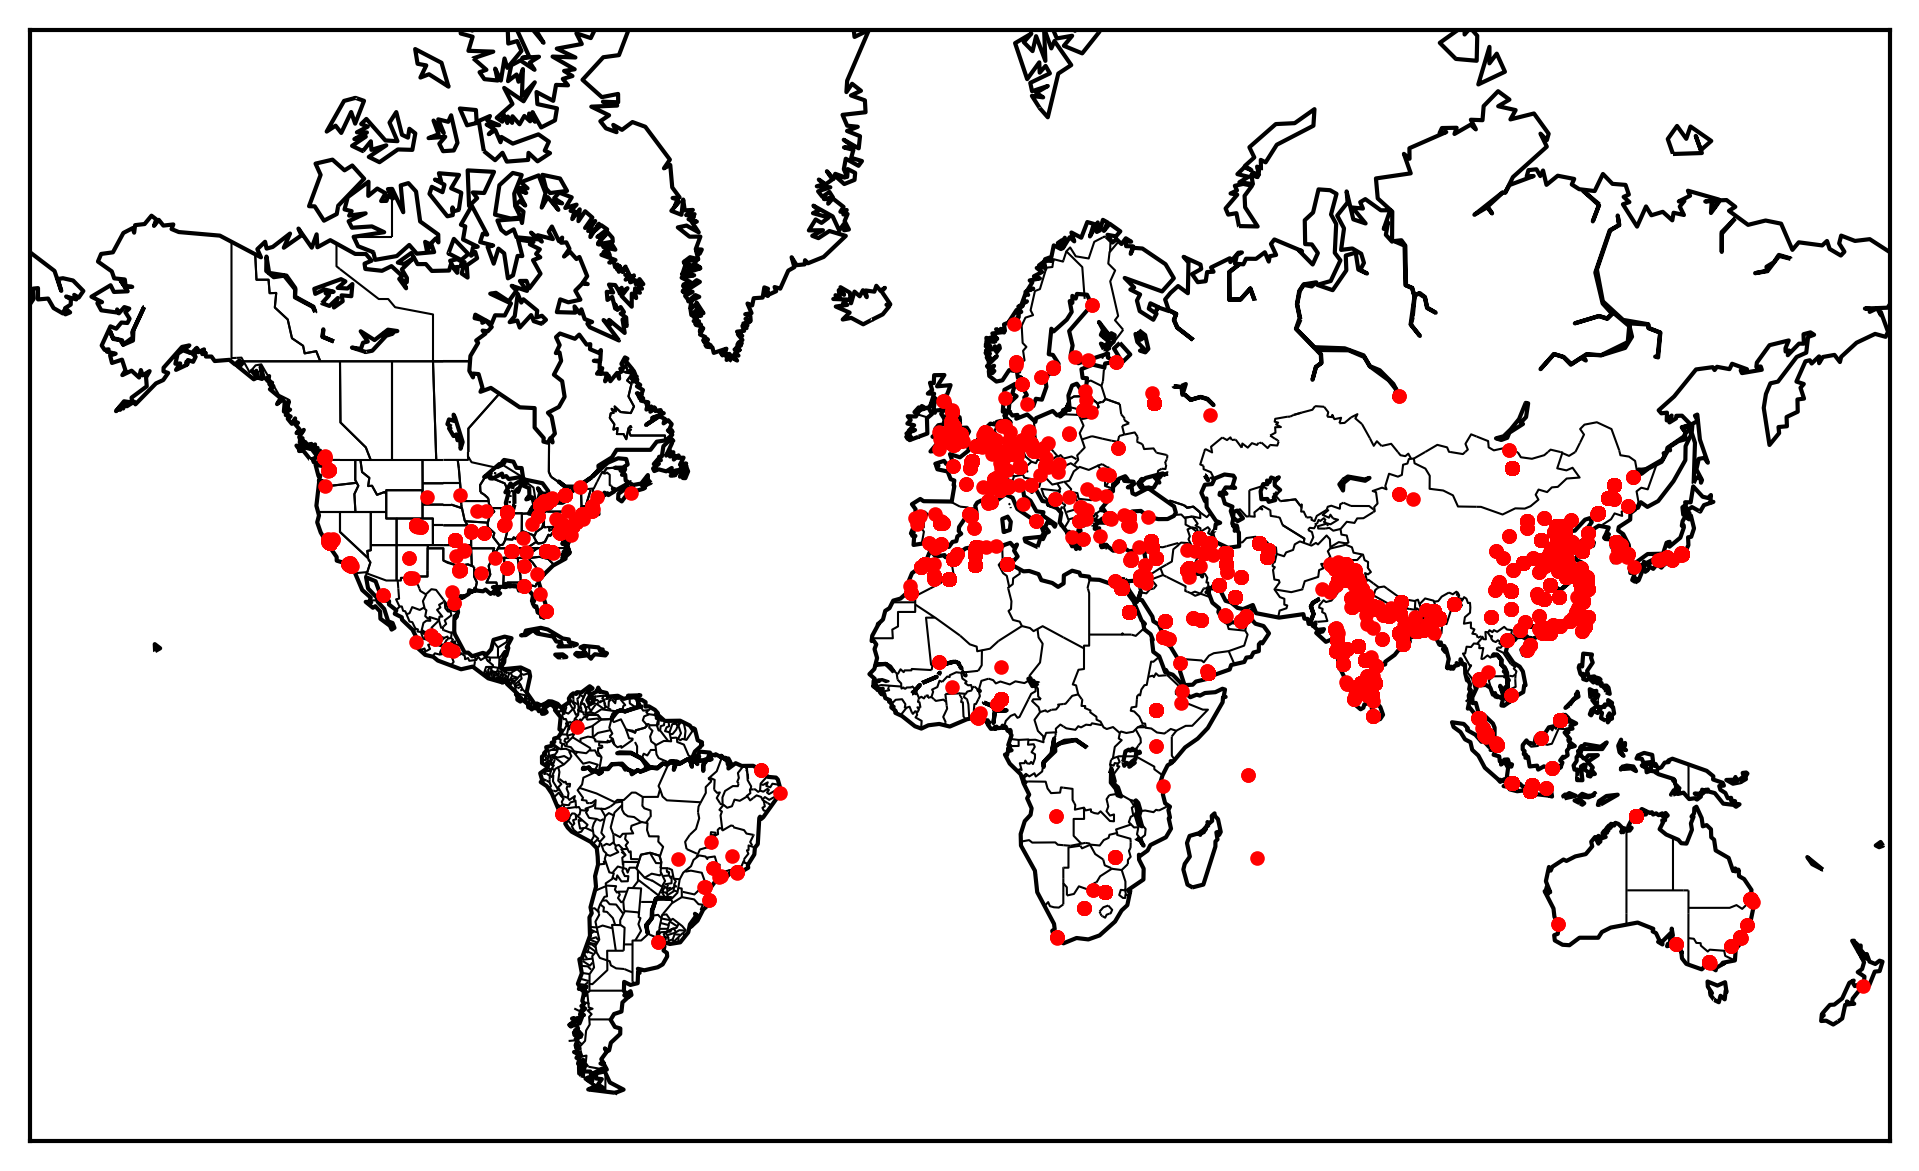
\includegraphics[width=0.48\textwidth]{./images/map.png}
%  \end{center}
%  \caption{Birds}
%\end{wrapfigure}


\begin{figure}
\centering
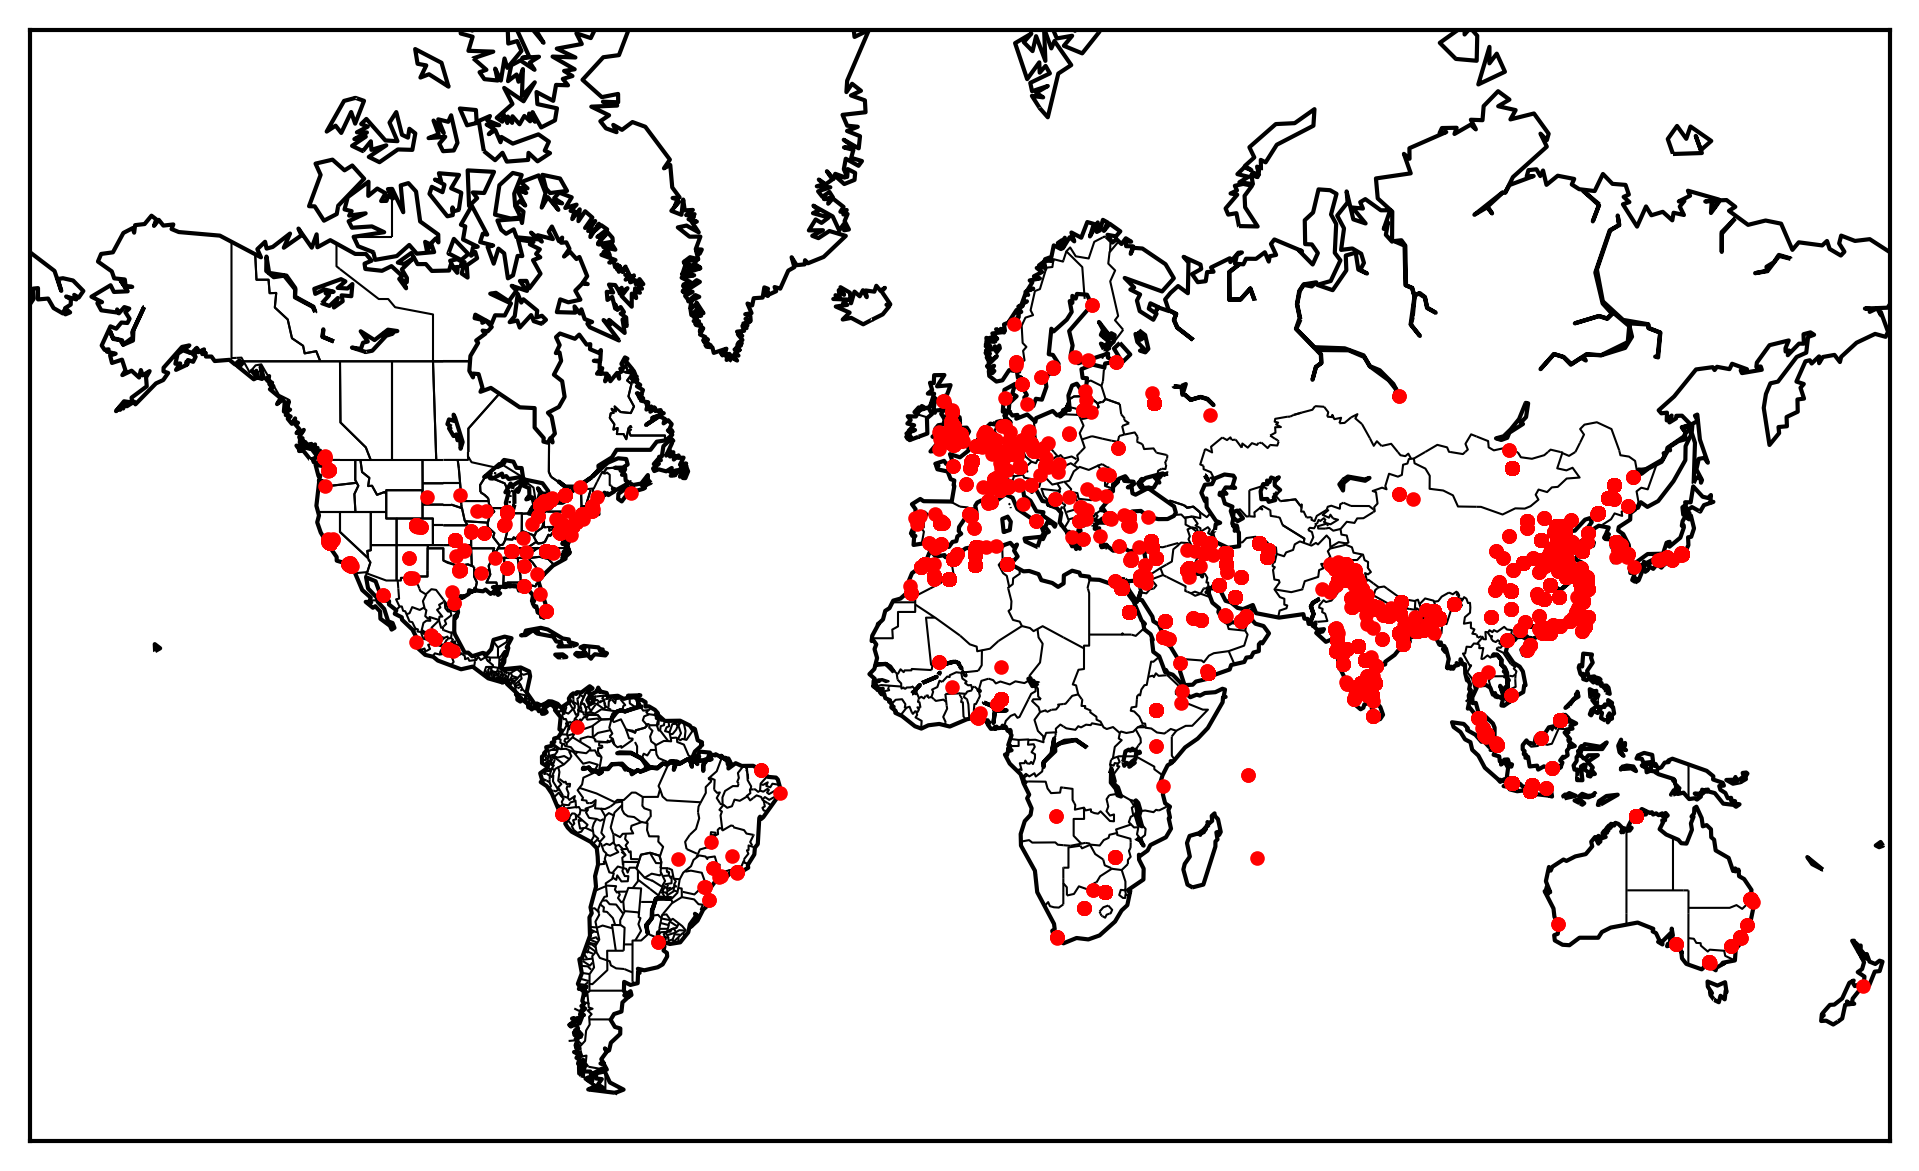
\includegraphics[width=0.5\textwidth]{./images/map.png}
\caption{A map of locations where gpvdm has been downloaded.}
\label{fig:downloadmap}
\end{figure}

\begin{figure}
\centering
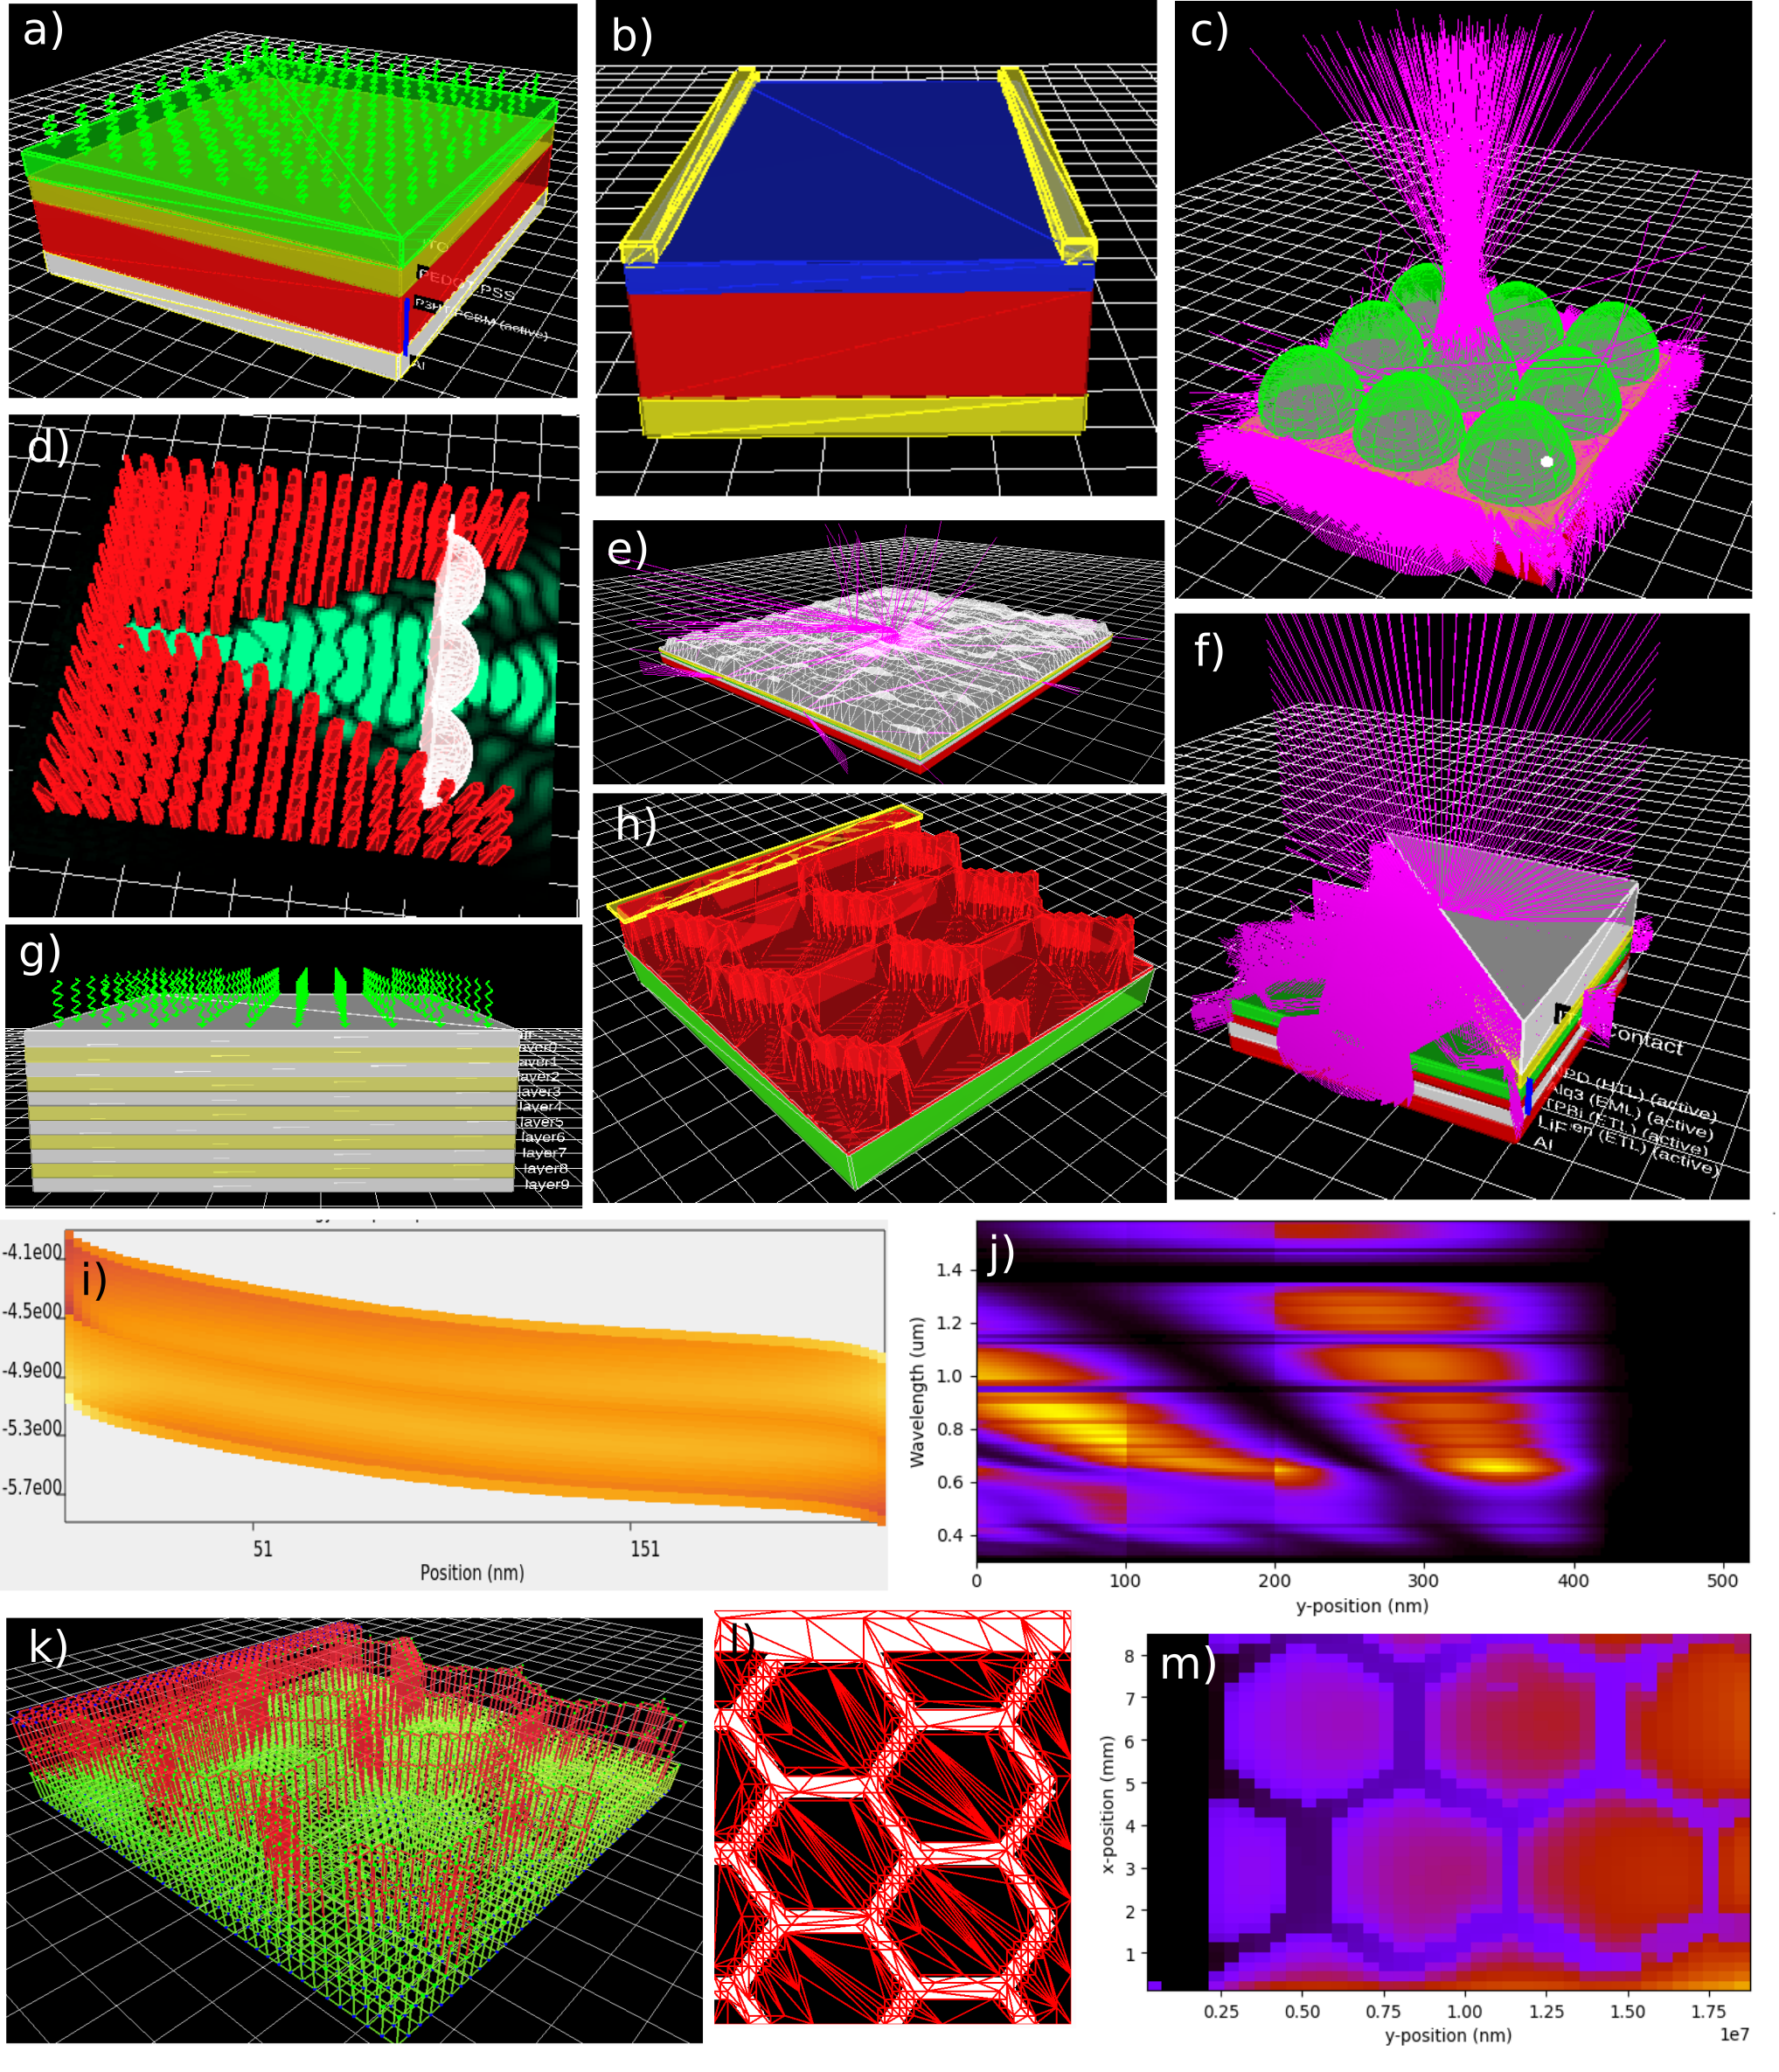
\includegraphics[width=0.9\textwidth]{./images/all_devices.png}
\caption{a); Organic/Perovskite solar cell simulation; b) OFET transistor simulation; c) Microlens simulation; d) Photonic waveguide simulation; e) light escaping structured films; f) OLED simulation; g) Optical filter simulation; h) large area device modelling (hexogonal contacts); i) Mapping carrier density in position/energy space; j) Building complex 3D meshes; and k) resistance maps of large area devices.}
\label{fig:alldevices}
\end{figure}

\section{Why gpvdm?}
By burning fossil fuels we are releasing $\sim 33.3$ gigatonnes of $CO_2$ per year \cite{Liu2022} and thus humanity is steadily changing the composition of Earth's atmosphere. Since 1960, $CO_{2}$ in the atmosphere has risen by around \href{https://gml.noaa.gov/ccgg/trends/}{30\%} this in turn is increasing average global temperatures\cite{ManabeandWetherald} and making our home planet Earth, a more difficult place to live on. We therefore have two choices, either cut emissions or face an existential crisis. Thin film devices such as solar cells and OLEDs offer a viable way to reduce our $CO_{2}$ emissions, either by providing low carbon electricity, or providing an efficient way to use the energy once generated. It is therefore important that technologies based on thin film devices continue to be developed and succeed. By developing and releasing \href{www.gpvdm.com}{gpvdm}, I hope, I am enabling scientists throughout the world to understand these devices a little bit better, which I hope will contribute in a very small way to solving our climate crisis.

Solar cells and OLEDs happen to come from a class of devices called diodes. This class of devices has many uses including optical sensors, medical sensors, switches, rectifiers. Thus as a pleasant side effect of gpvdm the development of these devices is also being helped.

\section{About this book/manual}
This manual is (in the end) intended to be the definitive guide to simulating devices with gpvdm. The idea is that one will be able to read this book and learn in a step by step way how to simulate many modern opto-electronic devices.  However, not all aspects of this book are yet finished. I therefore recommend you also watch the \href{https://www.youtube.com/channel/UCbm_0AKX1SpbMMT7jilxFfA}{YouTube} channel (and subscribe! ;)) where I describe many of the features in more detail and give demonstrations on the use of gvpdm. I would suggest you treat the videos as lectures (and take notes) rather than entertaining videos (well I hope they are entertaining too!). New releases are generally announced on \href{https://twitter.com/gpvdm_info}{Twitter}, which I also suggest you follow the gpvdm account and make sure you are using an up-to date version. I often release version every week.  Please read papers which were published from this model - do also read the supplementary information (SI) to the papers, as I often write about the model in there.
This book starts off with explaining how to simulate organic solar cells. This is because organic solar cells are the easiest class of device to simulate, it then moves onto Perovskite devices, and OLEDs. More complex classes of devices follow.  If you are new to simulation work or in indeed gpvdm, I suggest you start with the first chapters and work your way to the more complex devices.

\section{What is the history of gpvdm?}
I started writing gpvdm just after finishing my PhD in 2009 while taking a break for academia and deciding what to do next. At that time it was a simple drift diffusion diode model which did not take account of disorder. The majority of the complex core of gpvdm which deals with disordered materials was written while I was working in the Physics Department at the Imperial College London in 2010-2011. During this time I was working for Jenny Nelson on organic solar cells, it was a very productive and exciting time. Since then the model has been expanded to model many other classes of material system and classes of devices. Since 2009 thousands of people have downloaded gpvdm and \href{http://www.gpvdm.com/publications.html}{hundreds (the list is by definition always out of date)} of people have published their own papers using the model.

\section{What is the roadmap for gpvdm?}
The aim is to make gpvdm a completely general opto-electronic model which can be used by anyone to learn about and explore the world of novel opto-electronic devices.  I want gpvdm to be an engine which people can use to push their own research forward and for education. The exact road map on how to get there is not defined.  As collaborators contact me asking for new features I add them, what comes first depends on what people want.. I never view gpvdm as finished, and release improvements in small increments, therefore if you discover and report a bug, check back in a week or so to see if it is fixed in the next version.  The same goes for this book, it evolves weekly as I write it. So if a section is missing, check back next week it might be finished.

\section{Using gpvdm in industrial/academic work}
\label{sec:using_gvpdm}
You are free to use gpvdm in industrial/academic work. In fact, I'm super happy if you use it in your work, papers or books. However, the following further conditions apply:\\\\
1. If you use gpvdm to generate results, then clearly say so in your work. This can be as simple as one sentences saying: "we used gpvdm to perform the simulations" \\\\
2. If you publish a book, paper or thesis where gpvdm has been used you must cite at least three papers associated with the model.  To find out which papers to cite, click on the area indicated in red in figure \ref{fig:cite_me} when using the model.   You are free to choose which papers to cite but PLEASE do not cite the manual. I can't include the manual in paper lists when applying for funding.\\
\\
I ask you to do this because citations are an easy way to demonstrate that people are using gpvdm. Demonstrating use is key to finding money/people to continue the development of gpvdm.  So by doing this you are guaranteeing the future of gpvdm and its continued availability for others.  Thank you!


\begin{figure}[H]
\centering
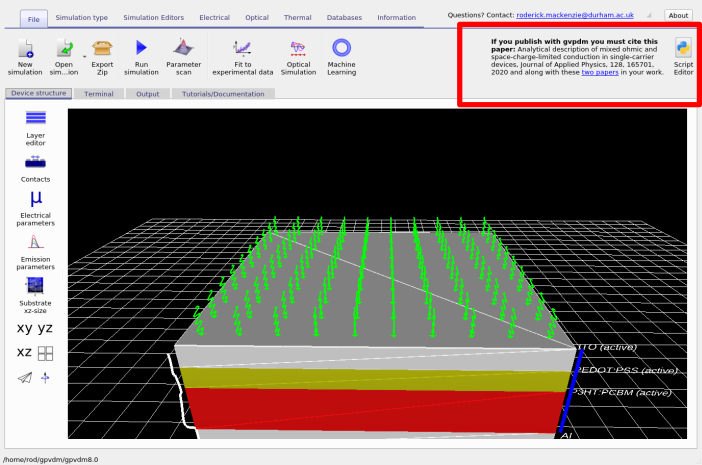
\includegraphics[width=0.7\textwidth]{./images/cite_me2.png}
\caption{If you click on the area indicated by the red box, the model will tell you which papers should be cited.}
\label{fig:cite_me}
\end{figure}

\section{Bugs}
I get quite a lot of feature requests from people wanting features added or for bugs to be fixed. I really appreciate the feedback!  However, I am currently employed at a UK University and my time is split between teaching, research and admin. My performance in my job is measured by the number of high impact papers I push out per year. I therefore have to prioritize feature requests and bug fixes for people who would like to write a paper with me (i.e. my collaborators).... Therefore if you would like:

\begin{itemize}
  \item A bit of advice on how to do x or y with the model then please do feel free to shoot me a mail, and I will do my best to get back to you. If you don't hear back from me just send the mail again.. I get loads of e-mails, and things get lost if I don't answer quickly.
  \item If you want to report a bug, then please do that, and I will do my best to fix it in the next release. But I can't promise when it will be fixed.
  \item  If you would like a features added or a steady stream of help (i.e. you are asking for my time) then please consider inviting me to join in your work and collaborate on a joint paper. I am happy to add what ever feature you want to the model, or fix what ever bug you may have but in return I would ask for the inclusion of my name on the author list. By doing this it makes it much easier for me to justify sinking time into your project.
\end{itemize}
    
If you don't need help from me to use gpvdm then please feel free to do what you want with the results - no need to contact me.

\section{Installing gpvdm}

\subsection{Windows (if you have admin rights)}
Go to the download page for gpvdm at \url{http://www.gpvdm.com/windows.php} and download the latest version.  Simply double click on it and say yes to all questions.  In general I release a new version every couple of weeks and it's worth keeping your version up-to-date. On modern versions of windows, windows will ask you if you want to install an unsigned executable from an unknown author, and warn you that this could damage your computer.  The reason you get this message is because I have not cryptographically signed the .exe file. I have not signed it because I do not own a private cryptographic key with which to do this.  To get such a key I would have to send my passport off to a key authority to prove who I am and then pay them 500 pounds/year for the privilege of them validating who I am.  Needless to say, that I am not very excited about paying 500 pounds/year so you will just have to click away the warnings from windows.

\subsection{Windows (No admin rights)}
If you don't have admin rights to your computer it can be hard to install new software, gpvdm offers the option of running gpvdm while not properly installed.  Download the zip file containing gpvdm from \url{https://www.gpvdm.com/download_no_admin.php}.  Once you have downloaded the zip archive, open the zip file and extract the folder $pub$ to c:\textbackslash . Then rename the folder to be calledc:\textbackslash gpvdm.  Once you have done this run the executable c:\textbackslash gpvdm\textbackslash gpvdm.exe (see figure \ref{fig:directory}).

\begin{figure}
\centering
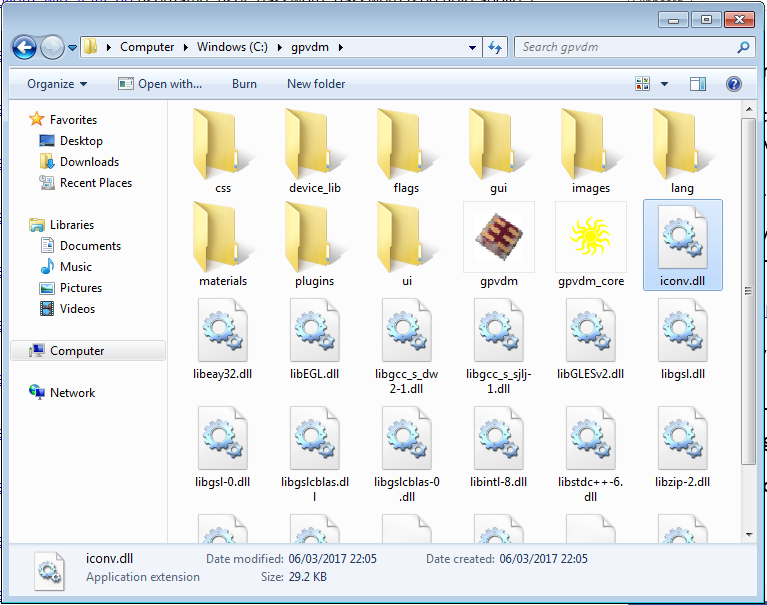
\includegraphics[width=70mm]{./images/dir.png}
\caption{Running and installing gpvdm.  Double click on the gpvdm icon to run the model.}
\label{fig:directory}
\end{figure}

%\subsection{Linux} \label{installing_on_linux}
%The windows version of gpvdm seems to be much more popular than the Linux version.  Therefore, I will tend to publish an updated windows exe every couple of weeks (along with the platform independent source code) and only publish updated linux rpms/deb packages when someone asks me to.  This means that the Linux deb/rpm files tend to lag behind the windows version by about a year.  For this reason I recommend you install the Linux version from source.


%\subsubsection{Linux from source the easy way}
%Download the gpvdm by issuing the command

%\begin{verbatim}
%git clone  https://github.com/roderickmackenzie/gpvdm
%\end{verbatim}
%Find your operating system in

%\begin{verbatim}
%build_system/dependency_scripts
%\end{verbatim}

%This script should install all the packages you need to run/compile gpvdm for a given OS. I don't always keep them up to date, so if you have a new version of an OS and the packages have been renamed you may have to hunt around.

%Then run:
%\begin{verbatim}
%./build
%\end{verbatim}

%Then select, (compile), and (auto). Then hit return to build.


%\begin{figure}[H]
%\centering
%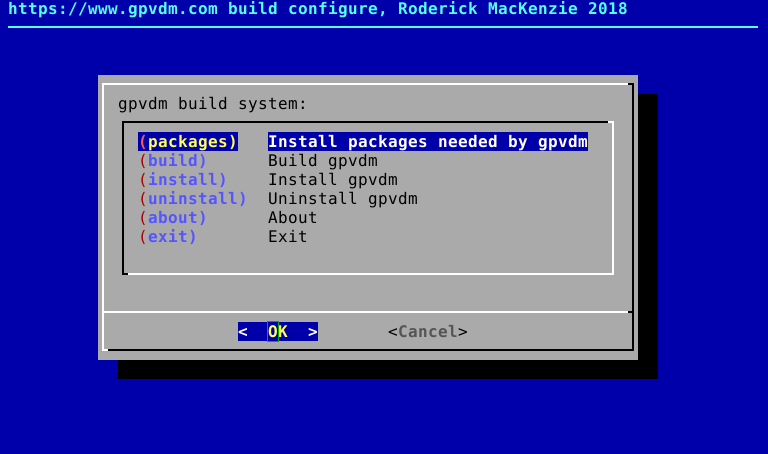
\includegraphics[width=0.7\textwidth]{./images/build.png}
%\caption{The linux build system, run ./build to get this menu.  }
%\label{fig:build}
%\end{figure}

